\begin{center}
\Huge
Vektorer og trigonometri
\end{center}

\section*{Enhedscirklen}
\stepcounter{section}

Trigonometri omhandler regning med trekanter. Til at regne på trekanter har vi såkaldte trigonometriske funktioner, der relaterer sidelængder og vinkler i retvinklede trekanter. De mest kendte trigonomestriske funktioner er I formentlig bekendte med: $\cos(v)$ og $\sin(v)$. Vi vil bruge enhedscirklen til at definere disse funktioner. Enhedscirklen kan ses af Fig. \ref{fig:enhed}
\begin{figure}[H]
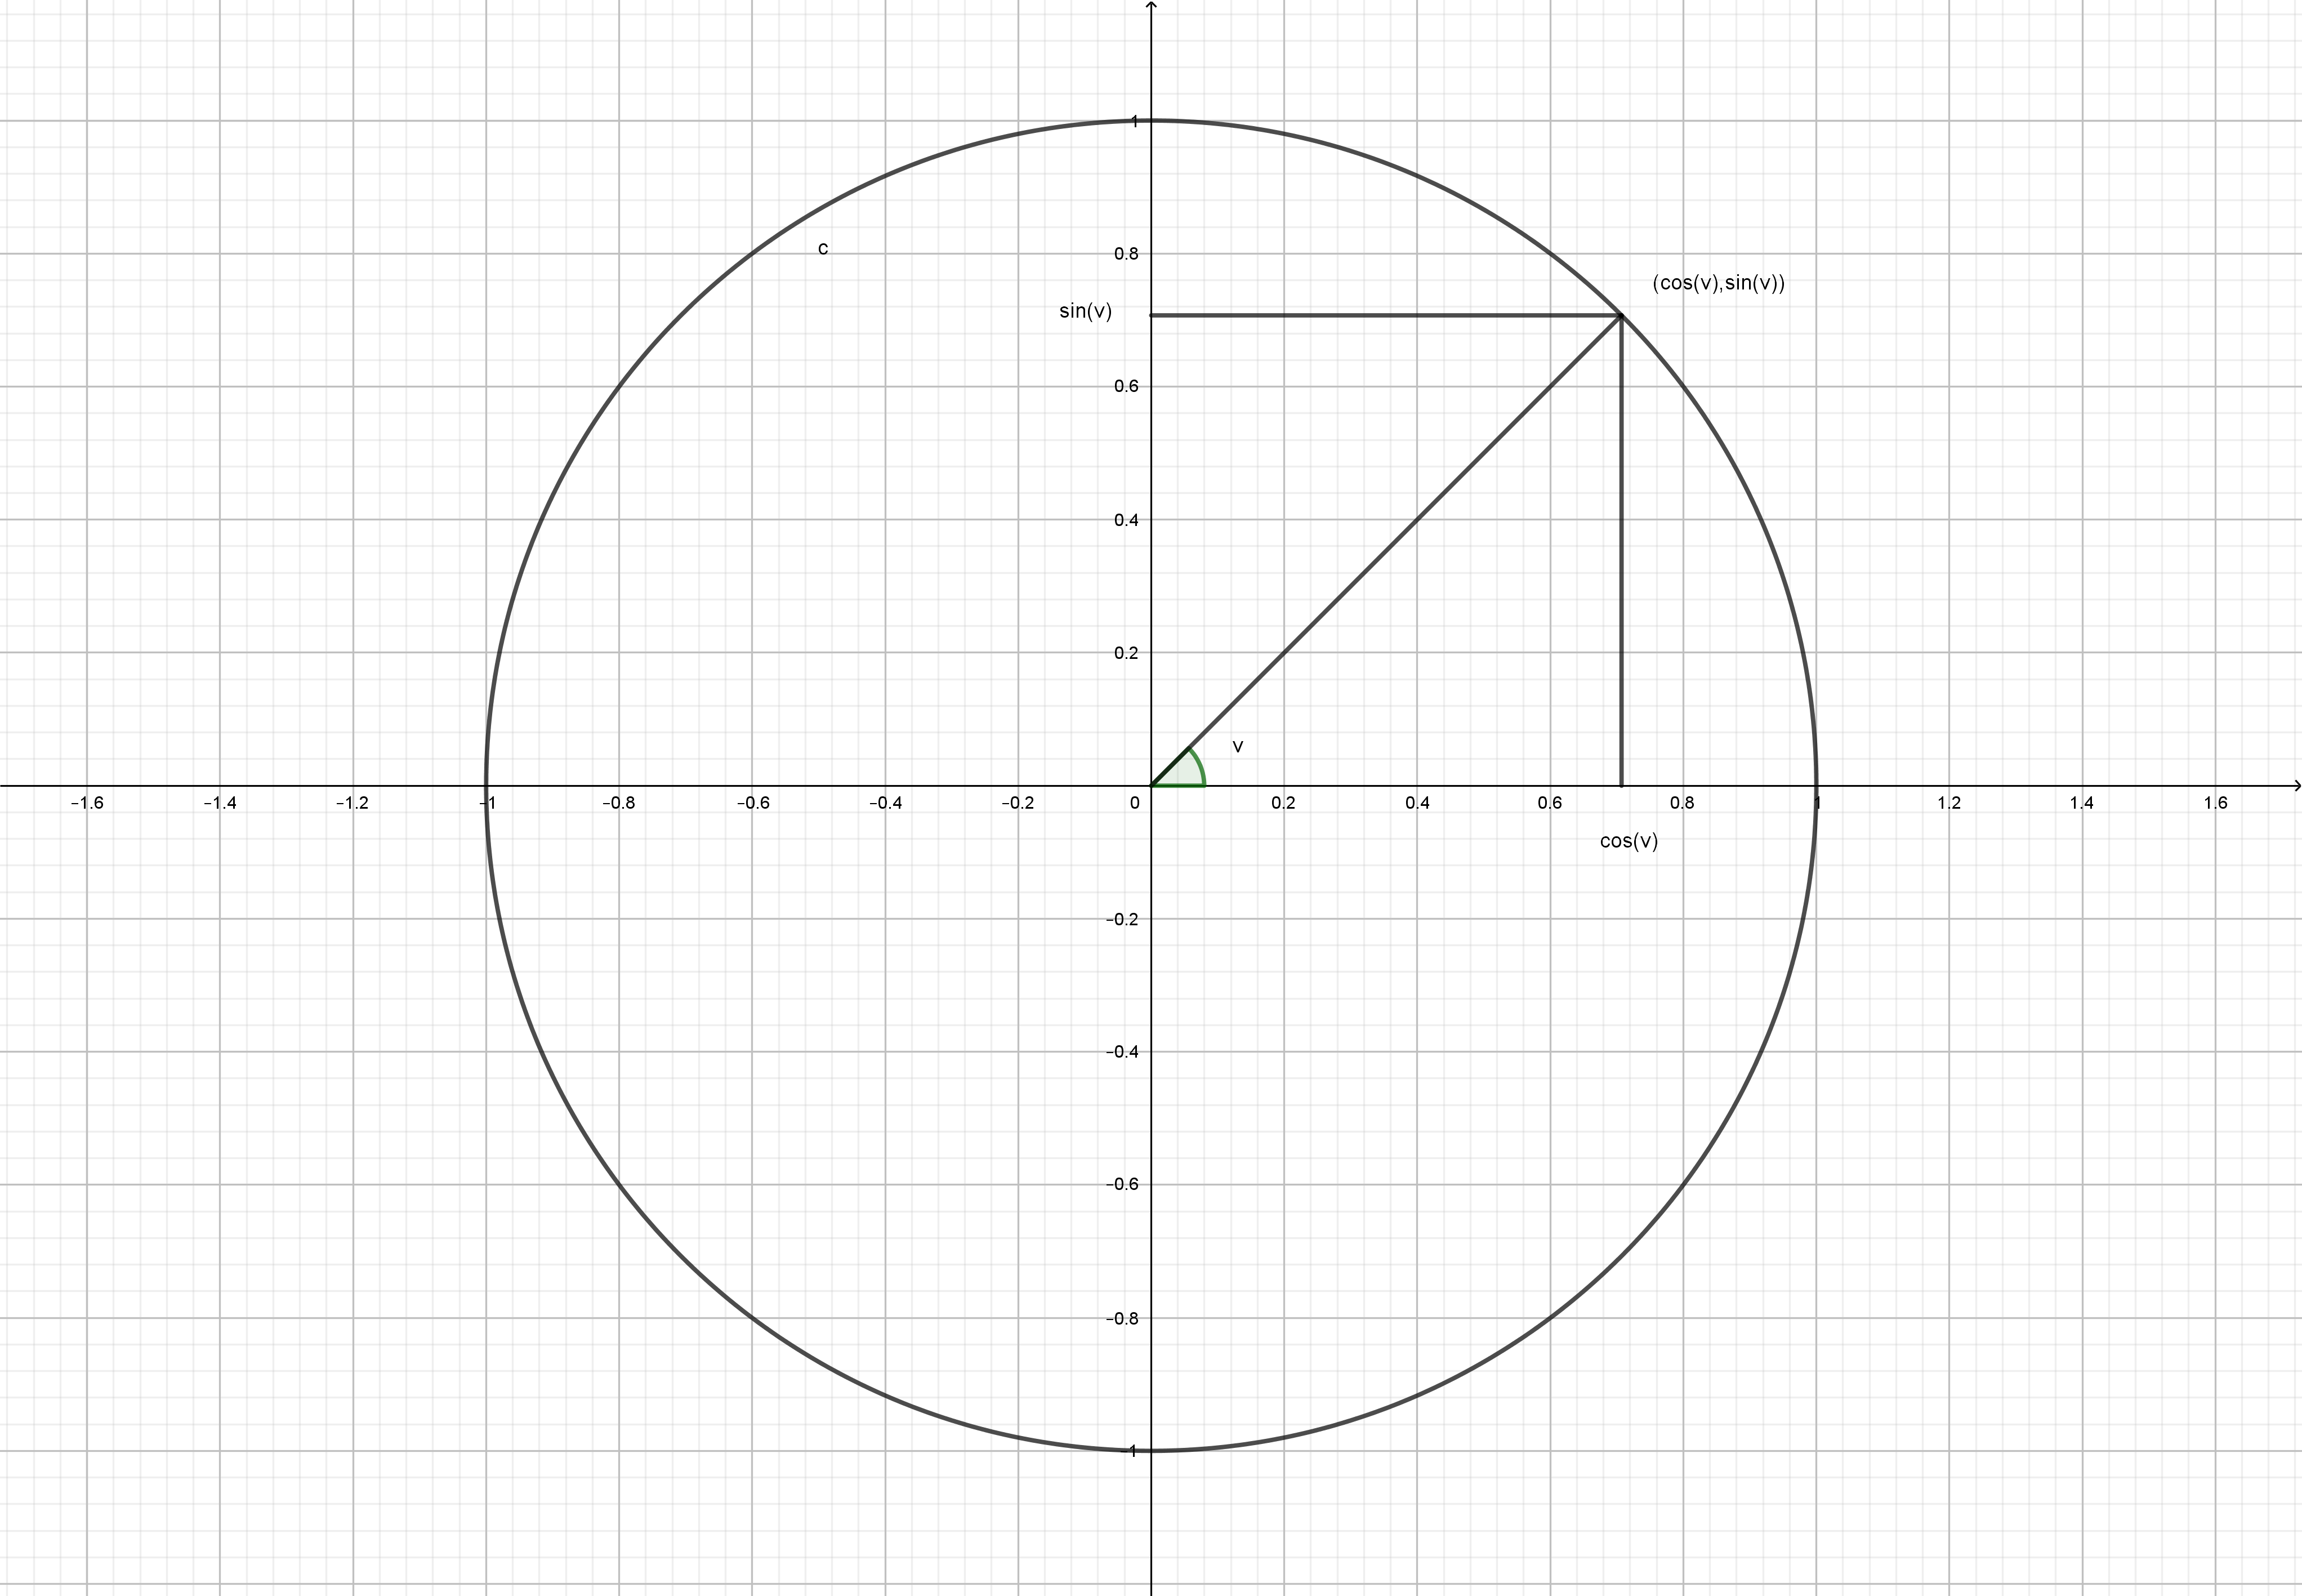
\includegraphics[width=\textwidth]{Billeder/enhedscirkel.png}
\caption{Enhedscirklen}
\label{fig:enhed}
\end{figure}
Enhedscirklen er en cirkel med centrum i origo og radius $1$. Vi kan bruge enhedscirklen til at definere $\cos$ og $\sin$.
\begin{defn}
Lad $P_v$ være et punkt på enhedscirklen, så vinklen mellem stedvektoren $\vv{OP_v}$ og $x$-aksen er $v$. Så defineres funktionerne $\cos(v)$ og $\sin(v)$ som koordinaterne til $P_v$:
\begin{align*}
P_v = (\cos(v),\sin(v)).
\end{align*}
\end{defn}

\begin{exa}
Det gælder, at $\cos(0) = 1$ og $\sin(0)=0$, da koordinatsættet til $P_0$ er 
\begin{align*}
P_0 = (1,0) = (\cos(0),\sin(0)).
\end{align*}
\end{exa}

\begin{setn}[Idiotformlen (den trigonometriske grundrelation)]
For enhver vinkel $v$ gælder der, at 
\begin{align*}
 \cos(v)^2 + \sin(v)^2 = 1.
\end{align*}
\end{setn}
\begin{proof}
Det er klart, at da enhedscirklen har radius $1$ og centrum i origo, så vil længden af alle vektorer på enhedscirklen have længde $1$. Tager vi stedvektoren $\vv{OP_v}$ og bestemmer længden får vi
\begin{align*}
1 = |\vv{OP_v}| = \left|\begin{pmatrix} \cos(v)\\\sin(v)\end{pmatrix}\right| = \sqrt{\cos(v)^2+\sin(v)^2}.
\end{align*}
Resultatet følger nu ved at opløfte begge sider af lighedstegnet i $2$.
\end{proof}

Tangens er den sidste trigonometriske funktion, vi skal betragte. Denne er defineret som 
\begin{align*}
\tan(v) = \frac{\sin(v)}{\cos(v)}.
\end{align*}
\section{Opgave 1}
Brug enhedscirklen til at aflæse $\cos(v)$ og $\sin(v)$ for følgende vinkler
\begin{align*}
&1) \ 90  &&2) \ 45   \\
&3) \ 180   &&4) \ 270   \\
&5) \ 60  &&6) \ 120   \\
&7) \ 360  &&8) \ 450   \\
\end{align*}

\section*{Opgave 2}
Afgør for hvilke vinkler $v$ og $w$, det gælder at
\begin{enumerate}[label=\roman*)]
\item $\cos(v) = \cos(w)$. 
\item $\cos(v) = \sin(w)$.
\item $\cos(v) = -\cos(w)$.
\item $\sin(v) = \sin(w)$.
\item $\sin(v) = -\sin(w)$.
\end{enumerate}

\section*{Opgave 3}
Brug idiotformlen til at bestemme $\cos(45)$ eksakt.

\section*{Opgave 4}
\begin{enumerate}[label=\roman*)]
\item Brug enhedscirklen til at argumentere for, at $\cos(30) = 0.5$.
\item Brug nu denne information samt idiotformlen til at bestemme $\sin(30)$.
\item Brug nu enhedscirklen til at bestemme $\sin(60)$ og $\cos(60)$. 

\end{enumerate}

\section*{Opgave 5}
Brug dit resultat fra Opgave 1 til at bestemme tangens for følgende vinkler
\begin{align*}
&1) \ 90  &&2) \ 45   \\
&3) \ 180   &&4) \ 270   \\
&5) \ 60  &&6) \ 120   \\
&7) \ 360  &&8) \ 450   \\
\end{align*}